%  LaTeX support: latex@mdpi.com
%  For support, please attach all files needed for compiling as well as the log file, and specify your operating system, LaTeX version, and LaTeX editor.

%=================================================================
\documentclass[remotesensing,article,submit,pdftex,moreauthors]{Definitions/mdpi}

%=================================================================
% MDPI internal commands - do not modify
\firstpage{1}
\makeatletter
\setcounter{page}{\@firstpage}
\makeatother
\pubvolume{1}
\issuenum{1}
\articlenumber{0}
\pubyear{2024}
\copyrightyear{2024}
%\externaleditor{Academic Editor: Firstname Lastname}
\datereceived{ }
\daterevised{ } % Comment out if no revised date
\dateaccepted{ }
\datepublished{ }
%\datecorrected{} % For corrected papers: "Corrected: XXX" date in the original paper.
%\dateretracted{} % For corrected papers: "Retracted: XXX" date in the original paper.
\hreflink{https://doi.org/} % If needed use \linebreak
%\doinum{}
%\pdfoutput=1 % Uncommented for upload to arXiv.org
%\CorrStatement{yes}  % For updates


%=================================================================
% Add packages and commands here. The following packages are loaded in our class file: fontenc, inputenc, calc, indentfirst, fancyhdr, graphicx, epstopdf, lastpage, ifthen, float, amsmath, amssymb, lineno, setspace, enumitem, mathpazo, booktabs, titlesec, etoolbox, tabto, xcolor, colortbl, soul, multirow, microtype, tikz, totcount, changepage, attrib, upgreek, array, tabularx, pbox, ragged2e, tocloft, marginnote, marginfix, enotez, amsthm, natbib, hyperref, cleveref, scrextend, url, geometry, newfloat, caption, draftwatermark, seqsplit
% cleveref: load \crefname definitions after \begin{document}

%=================================================================
% Please use the following mathematics environments: Theorem, Lemma, Corollary, Proposition, Characterization, Property, Problem, Example, ExamplesandDefinitions, Hypothesis, Remark, Definition, Notation, Assumption
%% For proofs, please use the proof environment (the amsthm package is loaded by the MDPI class).

%=================================================================
% Full title of the paper (Capitalized)
% \Title{Robot Team III: Scotty Strikes Back}
\Title{Visualization and Unsupervised Classification of Water Composition with UAV-based Hyperspectral Imaging and Generative Topographic Mapping}

% MDPI internal command: Title for citation in the left column
\TitleCitation{Title}

% Author Orchid ID: enter ID or remove command
\newcommand{\orcidauthorA}{0000-0002-5910-0183} % John
\newcommand{\orcidauthorB}{0000-0003-2688-648X} % Lakitha
\newcommand{\orcidauthorC}{0000-0002-9841-6703} % Shawhin
\newcommand{\orcidauthorD}{0000-0003-2657-3416} % Prabuddha
\newcommand{\orcidauthorE}{0000-0003-4265-9543} % David
\newcommand{\orcidauthorF}{0000-0003-0667-2345} % Ash
\newcommand{\orcidauthorG}{0000-0002-0126-218X} % Adam
% \newcommand{\orcidauthorH}{} % Gokul

% Authors, for the paper (add full first names)
\Author{John Waczak \orcidA{}, Adam Aker \orcidG{}, Lakitha O. H. Wijeratne \orcidB{}, Shawhin Talebi \orcidC{}, Ashen Fernando \orcidF{}, Prabuddha M. H. Dewage \orcidD{}, Mazhar Iqbal, Matthew Lary, David Schaefer, Gokul Balagopal, and David J. Lary *\orcidE{}}

%\longauthorlist{yes}

% MDPI internal command: Authors, for metadata in PDF
\AuthorNames{John Waczak, Adam Aker, Lakitha O. H. Wijeratne, Shawhin Talebi, Bharana Fernando, Prabuddha Hathurusinghe, Mazhar Iqbal, Matthew Lary, David Schaefer, Gokul Balagopal, and David J. Lary}

% MDPI internal command: Authors, for citation in the left column
 \AuthorCitation{Waczak, J.; Aker, A.; Wijeratne, L.O.H.; Talebi, S.; Fernando, B.; Hathurusinghe, P.; Iqbal, M.; Lary, M.; Schaefer, Balagopal, G.; D.; Lary, D.J.}
% If this is a Chicago style journal: Lastname, Firstname, Firstname Lastname, and Firstname Lastname.

% Affiliations / Addresses (Add [1] after \address if there is only one affiliation.)
\address[1]{%
Hanson Center for Space Sciences, University of Texas at Dallas, Richardson, TX 75080, USA;  john.waczak@utdallas.edu (J.W.); adam.aker@utdallas.edu (A.A.); lhw150030@utdallas.edu (L.O.H.W.); shawhintalebi@gmail.com (S.T.); ashen.fernando@utdallas.edu  (B.F.); pxh180012@utdallas.edu (P.M.H.D.); mazhar.iqbal@utdallas.edu (M.I.); MDL210001@utdallas.edu (M.L.); captdaveschaefer@gmail.com (D.S.); gokul.balagopal@utdallas.edu (G.B.);}

% Contact information of the corresponding author
\corres{Correspondence: david.lary@utdallas.edu} %; Tel.: (optional; include country code; if there are multiple corresponding authors, add author initials) +xx-xxxx-xxx-xxxx (F.L.)}


% Abstract (Do not insert blank lines, i.e. \\) 
\abstract{
Unmanned Aerial Vehicles (UAVs) equipped with hyperspectral imagers have emerged as an essential technology for the characterization of inland water bodies. The high spectral and spatial resolutions of these systems enable the retrieval of a plethora of optically-active water quality parameters via band ratio algorithms and machine learning methods. However, fitting and validating these models requires access to sufficient quantities of in situ reference data which are time-consuming and expensive to obtain. In this study, we demonstrate how the Generative Topographic Mapping (GTM), a Bayesian realisation of the Self Organizing Map (SOM), enables highly-detailed unsupervised classification and nonlinear endmember extraction of UAV acquired hyperspectral imagery. Specifically, the topographic relationship between classes maintained by the GTM presents an attractive alternative to other unsupervised approaches which do not provide a notion of similarity between learned classes. Using data collected across a North Texas pond, we apply the GTM to create a detailed map segmenting the area into distinct regions of interest. Further, by interpreting the learned classes as distinct endmembers, the GTM can be used to rapidly identify and map unique water constituents. We demonstrate this capability by using the GTM to map algal abundance as well as the dispersion of a rhodamine dye tracer released into the water.
}

% Keywords
\keyword{Hyperspectral Imaging; Remote Sensing; Unsupervised Classification; Endmember Extraction, Spectral Unmixing} 


%%%%%%%%%%%%%%%%%%%%%%%%%%%%%%%%%%%%%%%%%%
\begin{document}

%%%%%%%%%%%%%%%%%%%%%%%%%%%%%%%%%%%%%%%%%%
\section{Introduction}

Inland water bodies present a unique challenge to characterization by remote sensing imagery due to their complex spectral characteristics and small scale spatial variability. The broad bands of multi-spectral imagers coupled with the irregular shape of lakes and rivers results in pixels with highly mixed signals that are easily dominated by reflectance from shore and near-shore vegetation sources \cite{koponen2002lake, ritchie2003remote}. Recently, the combination of hyperspectral imaging with unmanned aerial vehicles (UAV) such as drones has emerged as a powerful approach to simultaneously address the spectral, spatial, and temporal limitations of traditional high-altitude and satellite-based collection \cite{adao2017hyperspectral,arroyo2019implementation}. UAV are significantly less expensive to deploy than their remote sensing counterparts, and low altitude flights enable centimeter-scale sampling while limiting the need for complicated atmospheric corrections \cite{banerjee2020uav}. However, the significant increase in data volume generated by these systems presents a new challenge, namely, how to efficiently extract water quality parameters of interest from intricate pixel spectra.

Significant research efforts have focused on the development of techniques and algorithms to retrieve water quality parameters from UAV-captured hyperspectral images (HSI). On-board compute installed alongside hyperspectral imagers can enable the rapid evaluation of spectral indices from HSI band ratios \cite{horstrand2019uav}. These band ratios and polynomial combinations of bands have been used to successfully invert optically-active water quality parameters such as turbidity directly from UAV acquired imagery \cite{vogt2016near, zhang2022selection}. Supervised machine learning techniques such as tree-based models, support vector machines, and neural networks have also been used to estimate a plethora of parameters such as colored dissolved organic matter, chlorophyll a, blue-green algae, and suspended sediment concentrations \cite{keller2018hyperspectral, lu2021retrieval}. The calibration and evaluation of these data-driven models demand a significant volume of coincident, in situ data. This can be addressed by coordinating UAV flights with reference data collection using autonomous robotic boats \cite{robot-team-1, robot-team-2}. Nevertheless, this approach relies on prior knowledge of expected sources in order to select appropriate reference instruments for model validation. The presence of unanticipated contaminants cannot be directly identified in this sensing paradigm. 

Extending the capabilities of UAV-based hyperspectral imaging to enable water quality monitoring in real-time scenarios where contaminant sources may not be known in advance requires two additional capabilities: dimensionality reduction techniques to permit the visual comparison of HSI, and endmember extraction techniques which can identify spectral signatures corresponding to unique sources within the imaging scene. In remote sensing where reference data are typically sparse, many approaches have been explored. For example, principal component analysis (PCA) and t-distributed stochastic neighbor embedding (tSNE) are dimensionality reduction methods commonly used to reduce HSI to two or three dimensions for visualization \cite{tyo2003principal,zhang2015hyperspectral}. Similarly for endmember extraction there are a variety of established approaches including geometric methods like vertex component analysis, statistical methods like k-nearest neighbors and non-negative matrix factorization (NMF), and deep learning methods based on autoencoder architectures \cite{heylen2014review,nascimento2005vertex, Feng2022HyperspectralUB, cariou2015unsupervised, su2019daen, borsoi2019deep, palsson2020convolutional}. Methods based on linear mappings like PCA and NMF are often too restrictive for HSI where the assumption of linear mixing is easily broken. However, the increased complexity of nonlinear methods like tSNE and autoencoders often lead to significant increases in computation time. An ideal approach should enable both visualization and nonlinear identification of relevant spectral endmembers.

% neurons that wire together, fire together
The self-organizing map (SOM) developed by Teuvo Kohonen is an unsupervised machine learning method which non-linearly maps high dimensional data to the nodes of a two-dimensional grid \cite{kohonen-som-1}. By preserving the topological relationship between nodes during training, the SOM ensures that similar spectral signatures are mapped together such that related HSI pixels naturally cluster together. This presents an attractive compromise by enabling the simultaneous visualization of HSI data and endmember extraction via the weight vector associated with each SOM node \cite{cantero2004analysis, duran2007time,som-hsi}. When reference data are available, the SOM can be utilized to provide semi-supervised labeling of HSI spectra \cite{riese2019supervised}. Furthermore, Danielsen et al. demonstrated that the dimensionality reduction offered by the SOM can even be used for on-board data compression of HSIs acquired by a CubeSat \cite{danielsen2021self}. Despite these clear capabilities, the SOM relies on a heuristic training algorithm with hyperparameters that can be challenging to tune and offers no direct probabilistic interpretation. To address these limitations, Bishop et al. developed the generative topographic mapping (GTM), a Bayesian latent-variable model inspired by the SOM \cite{gtm-bishop-1}. The GTM has been utilized in a variety of domains including drug design and chemical data visualization but has yet to see adoption for the analysis of hyperspectral imagery \cite{kireeva2012generative, gaspar2015chemical, horvath2019generative}.

In this paper, we explore the application of the GTM to UAV-acquired HSI for the characterization water quality. Using data collected at pond in Montague, North Texas, we first train a GTM using water-only pixels to produce a low-dimensional representation of the collected HSI. We use this mapping to explore the highly detailed small-scale variability within the pond and discuss how this can be used to guide reference data collection. Next, we demonstrate how the GTM can be utilized to identify relevant spectral endmembers from a combined dataset including land pixels, algae, water, and a simulated contaminant plume using a rhodamine tracer dye. Once identified, these endmembers can be used to rapidly map the abundance of spectral features within the pond. We demonstrate this capability by mapping the abundance of algae near the shore and to track the evolution of a rhodamine dye plume. 



%%%%%%%%%%%%%%%%%%%%%%%%%%%%%%%%%%%%%%%%%%
\section{Materials and Methods}


\begin{figure}[t]
%\begin{adjustwidth}{-\extralength}{0cm}
\centering
%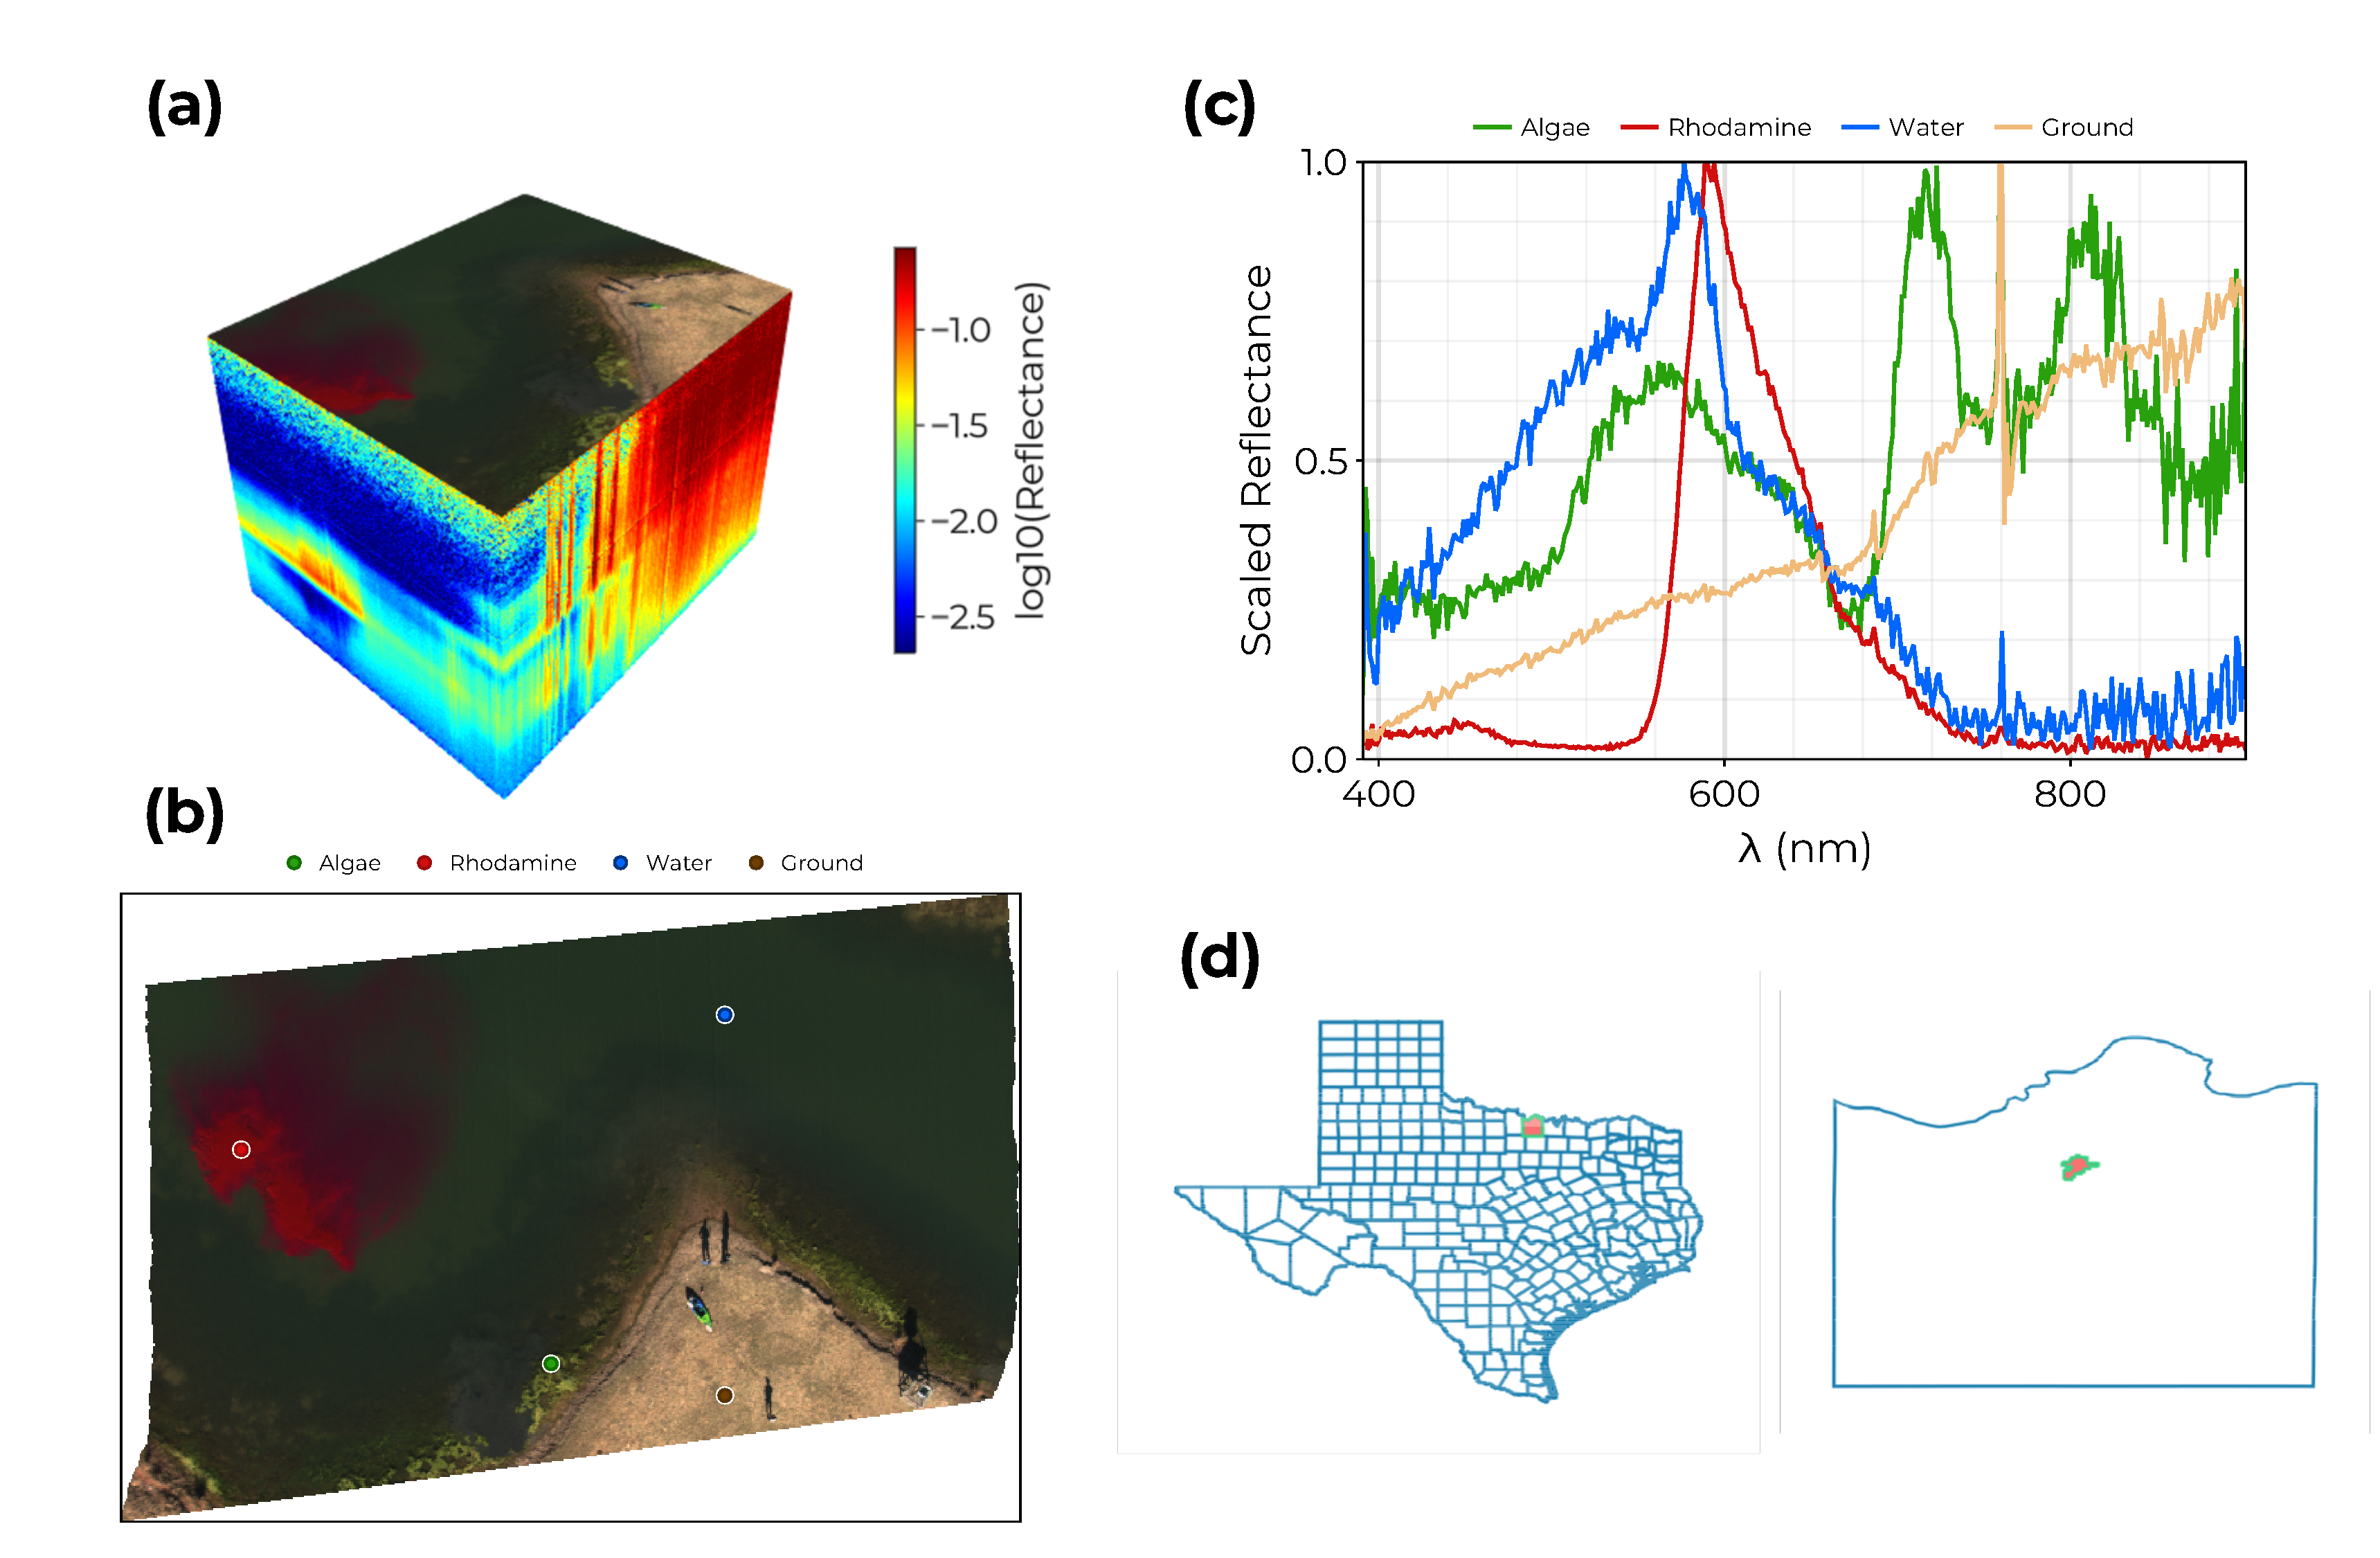
\includegraphics[width=15.5cm]{paper/figures/methods/sample-spectra.pdf}
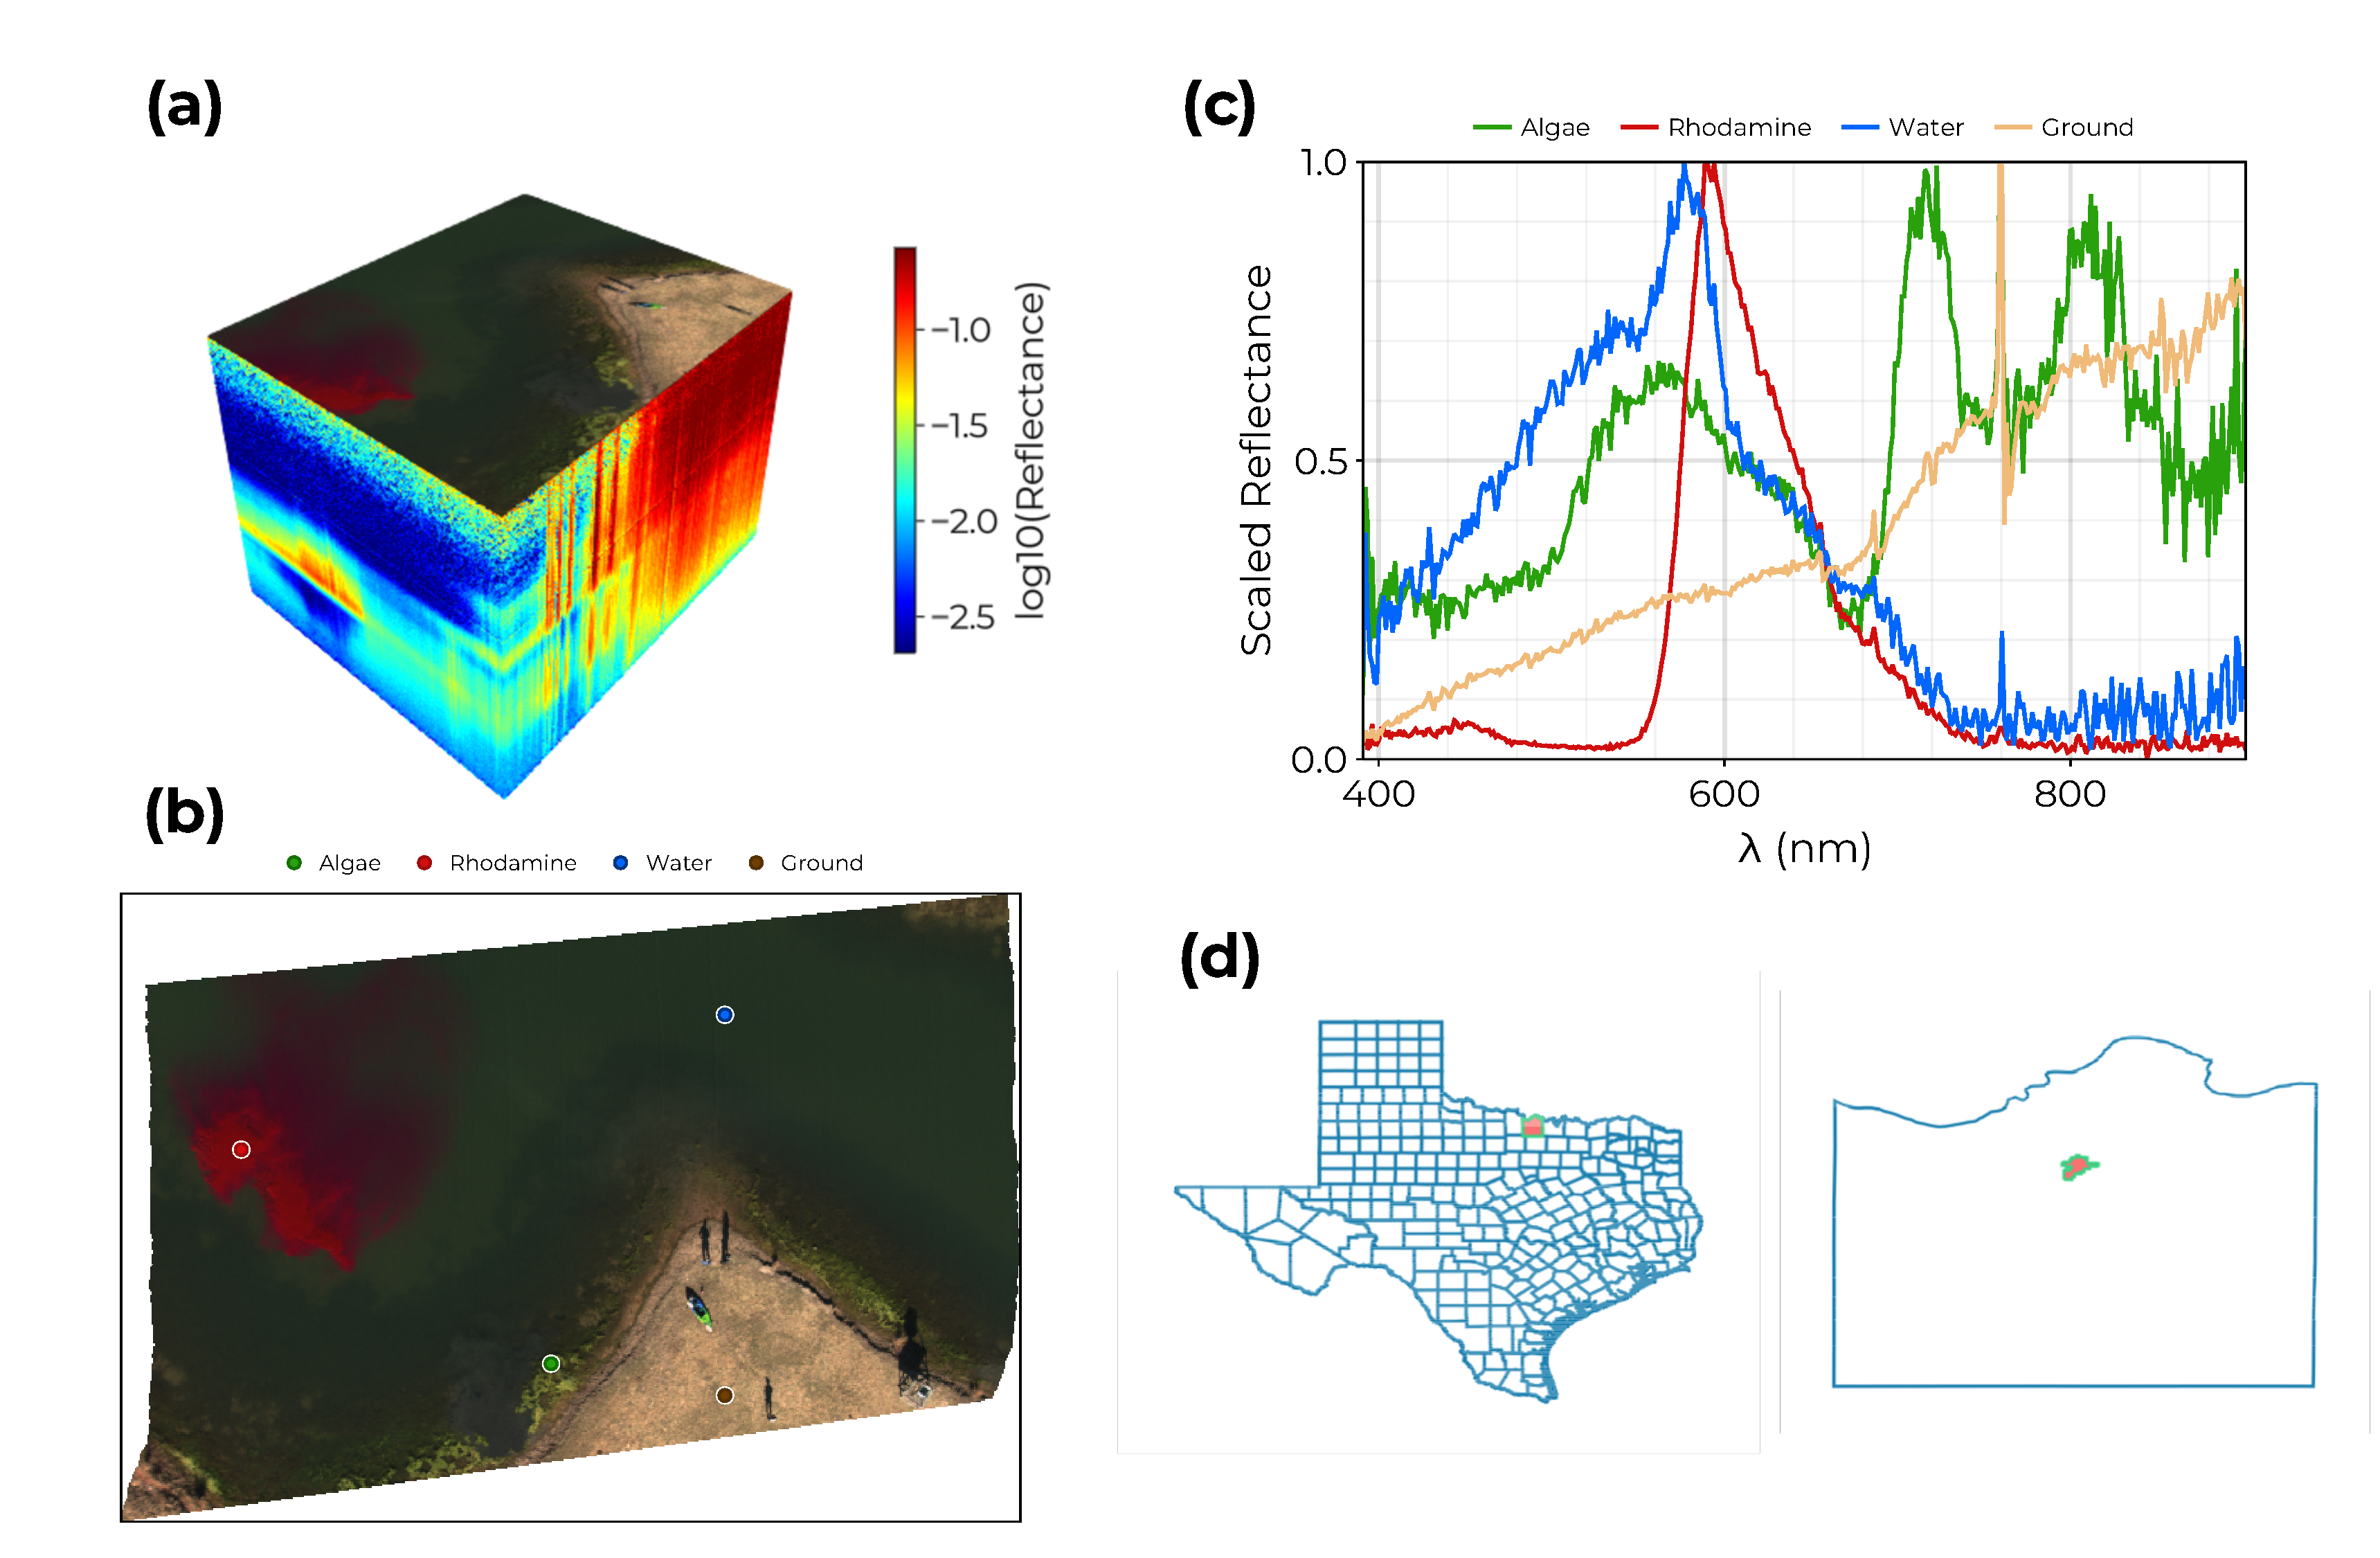
\includegraphics[width=\columnwidth]{paper/figures/methods/sample-spectra.pdf}
%\end{adjustwidth}
\caption{(\textbf{a}) Sample hyperspectral data cube. Spectra are plotted using their geographic position with the log10-reflectance colored along the z axis and a pseudo-color image on top. (\textbf{b}) Points taken from a sample hyperspectral data cube corresponding to algae, rhodamine dye, water, and dry grass. (\textbf{c}) Reflectance spectra for the exemplar points scaled so the peak value of each spectrum is $1.0$. (\textbf{d}) The location of the pond in Montague, Texas where data were collected for this study.\label{fig:sample-spectra}}
\end{figure}  


In this study, we explore the use of the GTM as a tool for dimensionality reduction and non-linear endmember extraction of hyperspectral imagery. To this end, a dataset of HSI were collected at a pond in Montague, North Texas (shown in panel d of Fig~\ref{fig:sample-spectra}) on 23 November 2020 using a UAV mounted hyperspectral imager configured as described in \cite{robot-team-1, robot-team-2}. In this section we first provide a detailed overview of the GTM algorithm. Next we describe the UAV platform used for HSI collection and the various steps used to processes captured HSI. Finally, we describe the GTM training procedure, hyperparameter optimization, and subsequent visualization methods used to analyze trained GTM models in this study.

%%% --- Generative 0Topographic Mapping ------------------------------------
\subsection{Generative Topographic Mapping}


The GTM is a probabilistic latent variable model inspired by the SOM for visualizing and clustering high-dimensional data. Like the SOM, the GTM assumes vectors $\mathbf{x}$ in the high-dimensional data space (here representing reflectance spectra) are constrained to a low-dimensional embedded manifold. The SOM describes this manifold using a regular grid of nodes, each having an associated weight vector defining the mapping from the manifold to the data space. The position of each data record $\mathbf{x}$ in the manifold is assigned as the position of the node whose weight vector has the minimum distance to $\mathbf{x}$. An iterative training procedure updates the weight vectors of each node to fit the manifold to the data such that nodes near each other in the SOM grid correspond to similar records (in the Euclidean sense) in the data space.

The GTM mimics the grid of the SOM by assuming data are generated from latent variables $\xi$ which are constrained to the $K$-many nodes of a regular grid. This assumption corresponds to establishing a prior distribution on the latent space of the form
\begin{equation}\label{eq:latent-prob}
    p(\xi) = \frac{1}{K}\sum_k^K \delta(\xi - \xi_k)
\end{equation}
where $\delta(\cdot)$ is the Dirac delta function.

Points $\xi$ in this latent space are mapped to the embedded manifold by a non-linear function $\psi$ parameterized by weights $W$. However, since real data is rarely noise-free, this embedded manifold will not be perfectly thin. To account for this the points $\xi$ are described in the data space by a radially symmetric Gaussian distribution, $\mathcal{N}(\psi(\xi),\, \beta^{-1})$, with mean $\psi(\xi)$ and variance $\beta^{-1}$. For a dataset consisting of $N$-many i.i.d. records, this choice yields a log-likelihood function of the form
\begin{equation}\label{eq:llh}
    \mathcal{L}(W, \beta) = \sum_n^N \ln \left(\dfrac{1}{K}\sum_k^K p(\mathbf{x}_n \mid \xi_k, W, \beta) \right)
\end{equation}
which can be maximized to fit $W$ and $\beta^{-1}$.

The function $\psi$ is typically chosen to be given by the sum of $M$-many radial basis functions (RBF) evenly distributed in the latent space so that $\psi(\xi) = W\phi(\xi)$ with centers $\mu_m$ and width $\sigma$ so that
\begin{equation}
    \phi_m(\xi) = \exp\left(-\dfrac{\lVert \xi - \mu_m \rVert^2}{2\sigma^2}\right).
\end{equation}
Together the number of RBFs, $M$, and $\sigma$ are hyperparameters for the model which govern the smoothness of the resulting manifold in the data space. Additionally, sparsity of $W$ can be controlled by an additional hyperparameter $\alpha$ corresponding to a prior distribution over the weights given by
\begin{equation}\label{eq:weight-prior}
    p(W \mid \alpha) =  \left( \frac{\alpha}{2\pi} \right)^{MD/2}\exp\left(-\frac{\alpha}{2}\left\lVert W \right\rVert_{F}^2\right).
\end{equation}

The use of RBFs for $\psi$ enables maximizing $\mathcal{L}(W,\beta)$ via an Expectation-Maximization routine. During each step of the fitting process, the responsibility of the $k$th node for the $n$th data record is computed as 
\begin{equation}\label{eq:responsibility}
    R_{kn} = p(\xi_k \mid \mathbf{x}_n, W, \beta) = \dfrac{p(\mathbf{x}_n \mid \xi_k, W, \beta)}{\sum\limits_{k'}^{K} p(\mathbf{x}_n \mid \xi_{k'}, W, \beta)}.
\end{equation}
Together these responsibilities form a matrix with entries $R_{kn}$ which are kept fixed during the maximization step. The maximization step is performed by updating the weights $W$ and variance $\beta^{-1}$ according to
\begin{align}\label{eq:m-step}
    W_{\text{new}} &= \left(\Phi^T G \Phi + \dfrac{\alpha}{\beta}I \right)^{-1} \Phi^T R X  \\
    \frac{1}{\beta_{\text{new}}} &= \frac{1}{ND} \sum\limits_{n}^{N} \sum\limits_{k}^{K} R_{kn} \left\lVert \psi_k - \mathbf{x}_n \right\rVert^2
\end{align}
where $\Phi_{km} = \phi_m(\xi_k)$, $X$ is the data matrix formed by concatenating the records $\mathbf{x}_n$, and $G$ is a diagonal matrix with $G_{kk} = \sum\limits_n^N R_{kn}$.



For this study, a freely available implementation of the GTM was developed in the Julia programming language \cite{gtm-code}. Julia is a dy

- GTM paper original \cite{gtm-bishop-1}
- GTM developments paper \cite{gtm-bishop-2}
- GTM code \cite{gtm-code}
- implementation designed to work in MLJ ecosystem \cite{blaom2020mlj}


at a pond in Montague, north Texas (shown in panel d of Fig~\ref{fig:sample-spectra})




\subsection{UAV-Based Hyperspectral Imaging}
A Freefly Alta-X autonomous quadcopter was used as a UAV platform for the robotic team.

The Alta-X is specifically designed to carry cameras and has a payload of up to 35 lbs. We equipped the UAV with a Resonon Pika XC2 visible+near-infrared (VNIR) hyperspectral imager. 

For each image pixel, this camera samples 462 wavelengths ranging from 391 to 1011 nm. 

Additionally, the UAV includes an upward facing Ocean Optics UV-Vis-NIR spectrometer with a cosine corrector to capture the incident downwelling irradiance spectrum.

Data collection by the hyperspectral imager is controlled by an attached Intel NUC small-form-factor computer. 

A second processing NUC is also included for onboard georectification and generation of data products.

The collected hyperspectral images (HSIs) are stored locally on a solid state drive that is simultaneously mounted by the processing computer.

- georetification \cite{muller2002program, baumker2001new, mostafa2000multi}

\subsection{Data Collection and Pre-Processing}
- Julia programming language used \cite{bezanson2012julia}



\subsection{Image Segmentation with the Normalized Spectral Similarity Score}


\begin{equation}
    \hat{\xi}_n = \sum_{k}^K R_{kn}\xi_k
\end{equation}



%%%%%%%%%%%%%%%%%%%%%%%%%%%%%%%%%%%%%%%%%%
\section{Results}

\subsection{GTM Fit}

\begin{figure}[t]
\centering
\includegraphics[width=0.8\columnwidth]{paper/figures/results/square-ndvi.pdf}
\caption{GTM Map: We plot the mean position of each data point in the latent space with points colored by the their associated NDVI values. The locations of the exemplar points for algae, rhodamine dye, water, and dry grass are shown in the latent space illustrating that the GTM has clearly distinguished land, near-land, and water pixels.\label{fig:}}
\end{figure}  


\subsection{Hyperparamter Optimization with BIC}


\begin{figure}[t]
%\begin{adjustwidth}{-\extralength}{0cm}
\centering
\includegraphics[width=\textwidth]{paper/figures/results/bic.pdf}
%\end{adjustwidth}
\caption{Results of the hyperparameter search. Left: Variation of BIC with $m$ and $s$ for fixed $\alpha=0.1$. Right: Variation of the BIC with with $m$ and $\alpha$ for fixed $s=1.0$. The white star in each plot indicates the parameters with the lowest BIC.\label{fig:hp-results}}
\end{figure}  


\subsection{Spectral Signatures}


\begin{figure}[t]
\begin{adjustwidth}{-\extralength}{0cm}
\centering
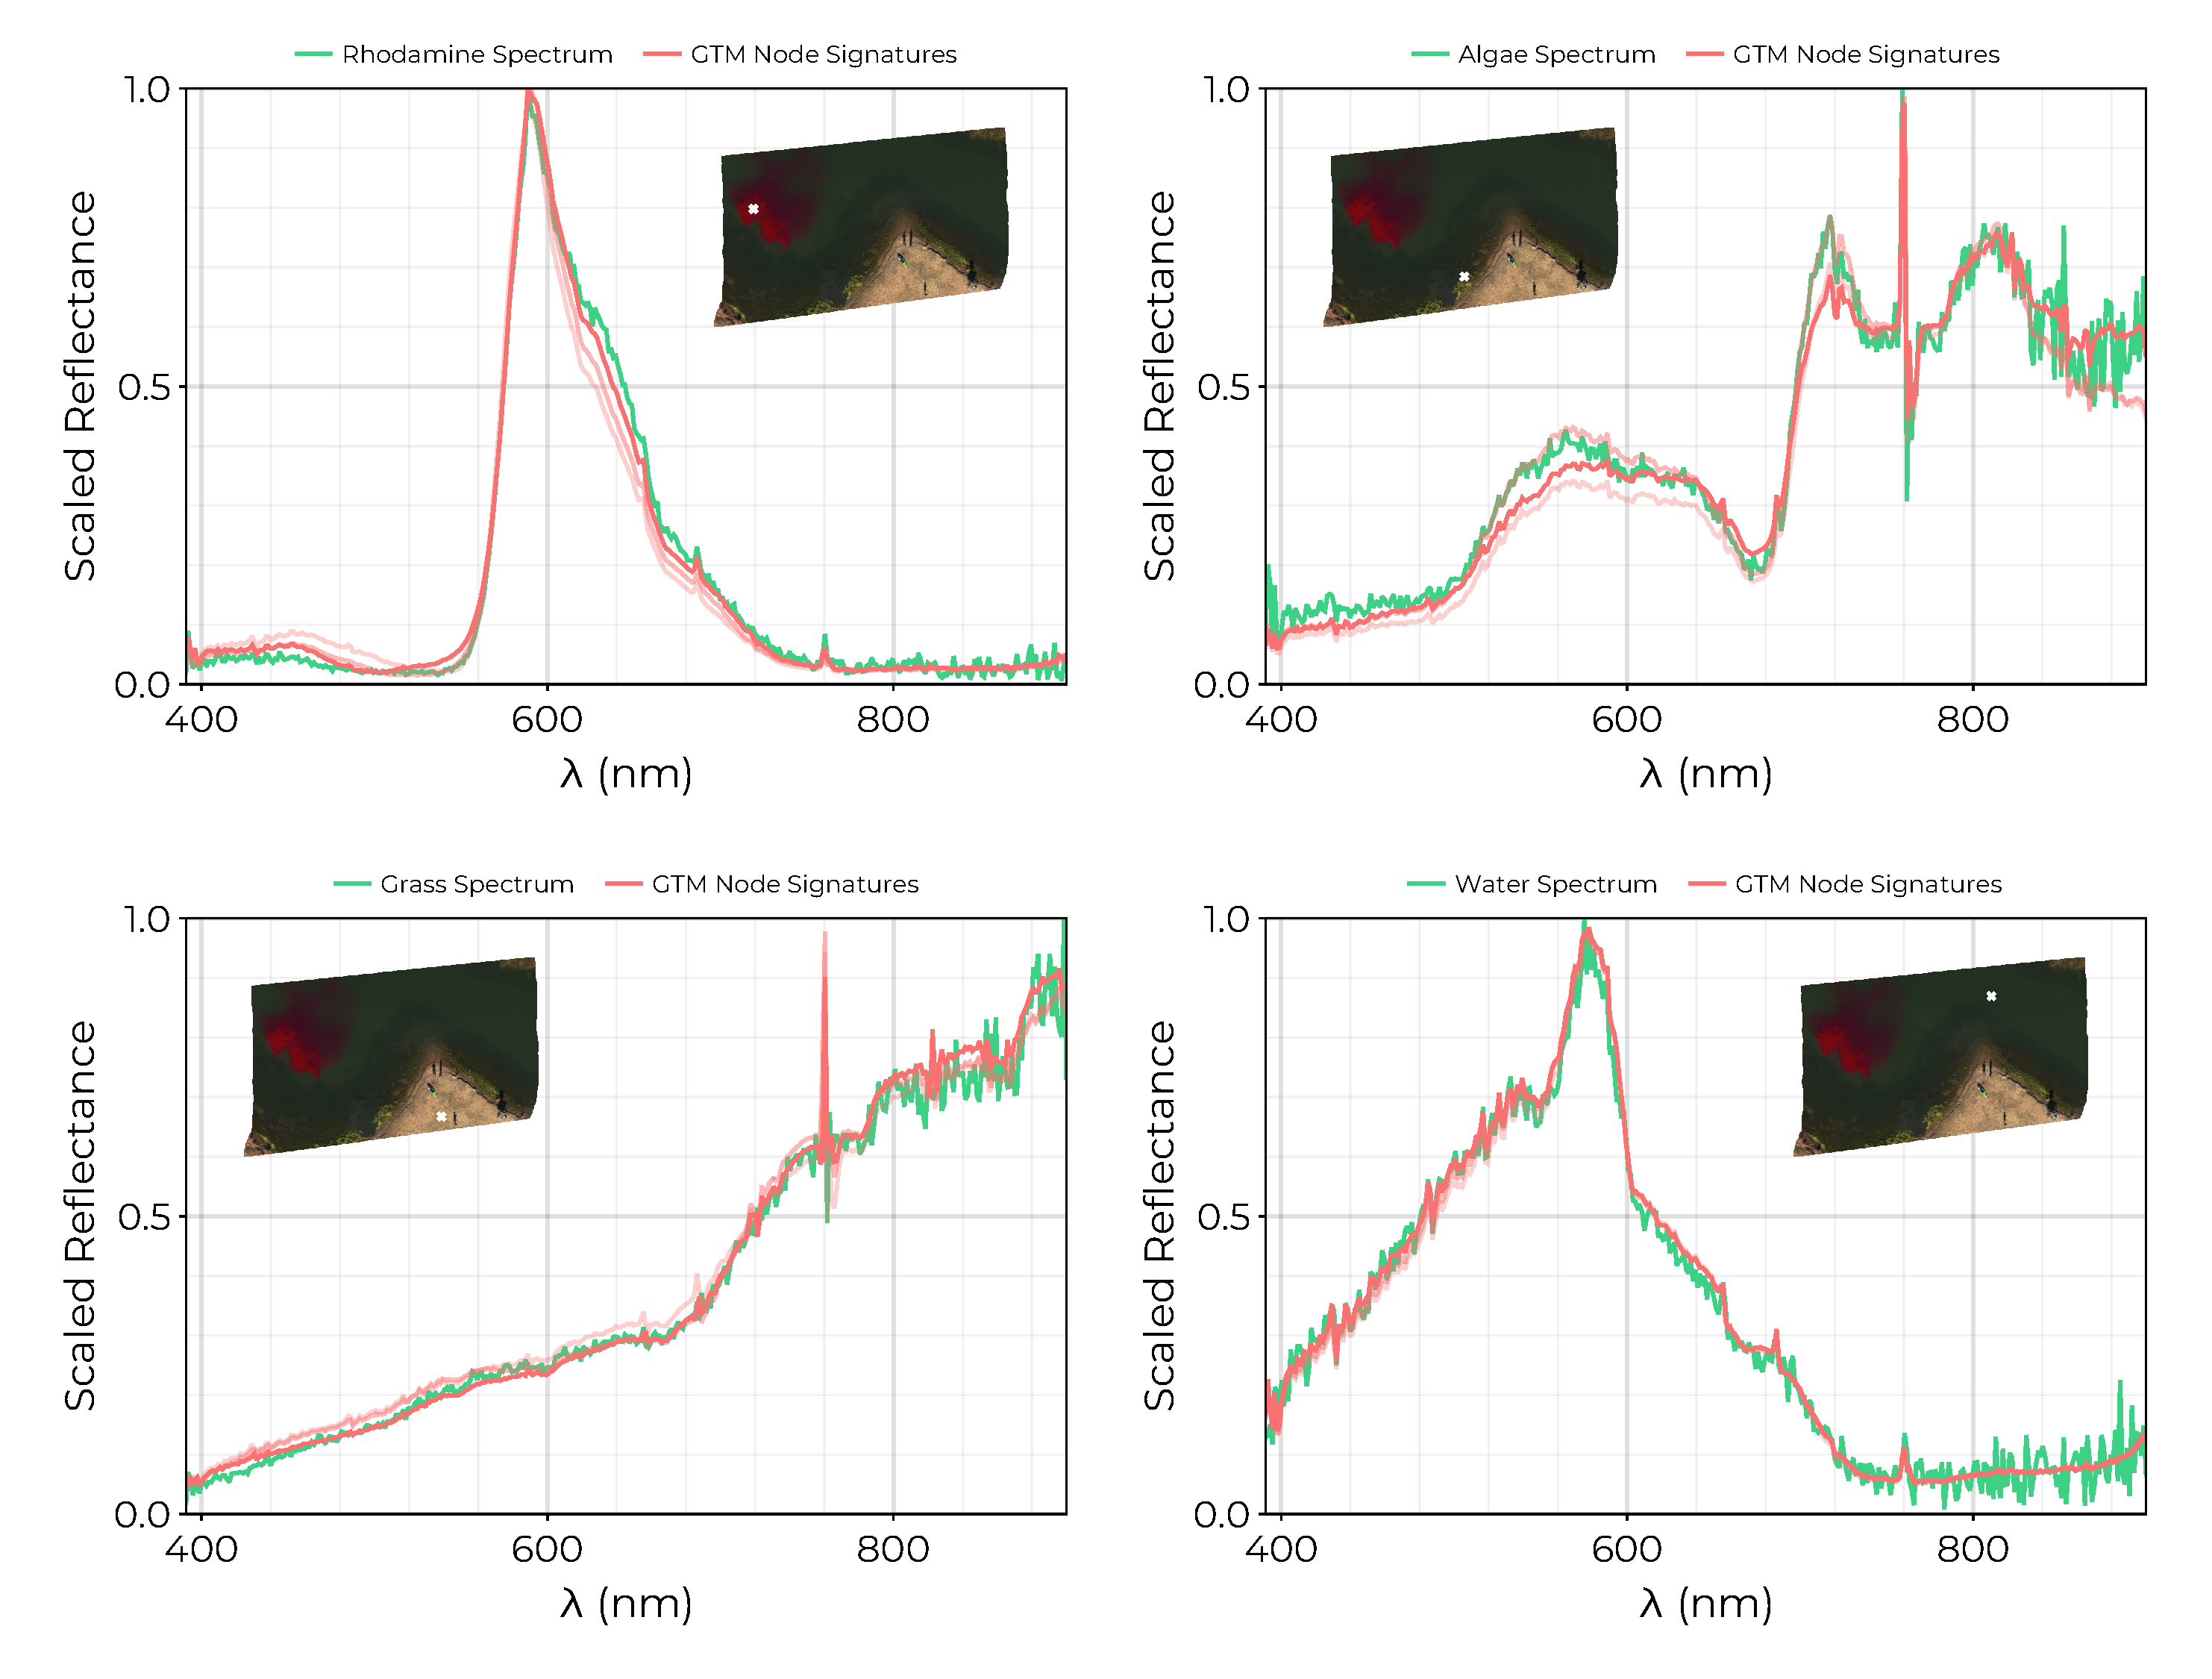
\includegraphics[width=15.5cm]{paper/figures/results/spectral-signatures.png}
\end{adjustwidth}
\caption{GTM Node Signatures corresponding to the exemplar spectra for the rhodamine plume (top left), algae (top right), dry grass (bottom left), and open water (bottom right). \label{fig:spectral-signautes}}
\end{figure}  

\subsection{Water Class Map}

\begin{figure}[t]
\begin{adjustwidth}{-\extralength}{0cm}
\centering
\includegraphics[width=18.0cm]{paper/figures/results/gtm-water.png}
\end{adjustwidth}
\caption{Classification map for GTM trained solely on water pixels (no land and no rhodamine plume). \textbf{(a)} GTM applied to all water pixels colored by their associated position in the latent space. \textbf{(b)} Representation of the poitns from the training set in the latent space. The points are colored with $\xi_1$ corresponding to red and $\xi_2$ corresponding to blue. \textbf{(c)} The associated GTM spectral signatures, $\Psi_i$, corresponding to the four corners and center of the GTM latent space. \label{fig:gtm-water}}
\end{figure}  


\subsection{Algae Identification}


\begin{figure}[t]
\begin{adjustwidth}{-\extralength}{0cm}
\centering
\includegraphics[width=15.5cm]{paper/figures/results/algae.png}
\end{adjustwidth}
\caption{\label{fig:algae-map}}
\end{figure}  



\subsection{Rhodamine Dye Plume Identification}

\begin{figure}[t]
\begin{adjustwidth}{-\extralength}{0cm}
\centering
\includegraphics[width=15.5cm]{paper/figures/results/rhodamine.png}
\end{adjustwidth}
\caption{\label{fig:rhodamine-map}}
\end{figure}  




%%%%%%%%%%%%%%%%%%%%%%%%%%%%%%%%%%%%%%%%%%
\section{Discussion}

\subsection{Summary of GTM applications in our paper}
\subsection{Comparison to other existing approaches in literature}
- Is there much done for classification in real time? 
\subsection{Comparison to Spectral Unmixing}
- Here we can re-interpret the GTM model as performing a type of Bayesian spectral unmixing and suggest how the method could be further extended to work in this domain. Critically, other traditional methods work by observing that pure endmembers form the vertices of a simplex. 

\subsection{Other applications of GTM}
- Discuss use of GTM means/modes/responsibilities feature transformer for supervised models (e.g. better than PCA) 
- Use of GTM classes to aid autonomous data collection by identification of "interesting" regons


- Drones can be equipped with HSI and compute to enable rapid generation of spectral indices like the NDVI for applications such as precision agriculture \cite{horstrand2019uav}

- Mention how Bishop suggests extensions to GTM for on-line learning which could be used to accelerate training for large HSI datasets


%%%%%%%%%%%%%%%%%%%%%%%%%%%%%%%%%%%%%%%%%%
\section{Conclusions}


%%%%%%%%%%%%%%%%%%%%%%%%%%%%%%%%%%%%%%%%%%
\vspace{6pt} 

%%%%%%%%%%%%%%%%%%%%%%%%%%%%%%%%%%%%%%%%%%
%% optional
%\supplementary{The following supporting information can be downloaded at:  \linksupplementary{s1}, Figure S1: title; Table S1: title; Video S1: title.}

% Only for journal Methods and Protocols:
% If you wish to submit a video article, please do so with any other supplementary material.
% \supplementary{The following supporting information can be downloaded at: \linksupplementary{s1}, Figure S1: title; Table S1: title; Video S1: title. A supporting video article is available at doi: link.}

% Only for journal Hardware:
% If you wish to submit a video article, please do so with any other supplementary material.
% \supplementary{The following supporting information can be downloaded at: \linksupplementary{s1}, Figure S1: title; Table S1: title; Video S1: title.\vspace{6pt}\\
%\begin{tabularx}{\textwidth}{lll}
%\toprule
%\textbf{Name} & \textbf{Type} & \textbf{Description} \\
%\midrule
%S1 & Python script (.py) & Script of python source code used in XX \\
%S2 & Text (.txt) & Script of modelling code used to make Figure X \\
%S3 & Text (.txt) & Raw data from experiment X \\
%S4 & Video (.mp4) & Video demonstrating the hardware in use \\
%... & ... & ... \\
%\bottomrule
%\end{tabularx}
%}

%%%%%%%%%%%%%%%%%%%%%%%%%%%%%%%%%%%%%%%%%%
\authorcontributions{FIXME}

\funding{FIXME}

\institutionalreview{Not applicable}

\informedconsent{Not applicable}

\dataavailability{We encourage all authors of articles published in MDPI journals to share their research data. In this section, please provide details regarding where data supporting reported results can be found, including links to publicly archived datasets analyzed or generated during the study. Where no new data were created, or where data is unavailable due to privacy or ethical restrictions, a statement is still required. Suggested Data Availability Statements are available in section ``MDPI Research Data Policies'' at \url{https://www.mdpi.com/ethics}.} 


\acknowledgments{In this section you can acknowledge any support given which is not covered by the author contribution or funding sections. This may include administrative and technical support, or donations in kind (e.g., materials used for experiments).}

\conflictsofinterest{Declare conflicts of interest or state ``The authors declare no conflicts of interest.'' Authors must identify and declare any personal circumstances or interest that may be perceived as inappropriately influencing the representation or interpretation of reported research results. Any role of the funders in the design of the study; in the collection, analyses or interpretation of data; in the writing of the manuscript; or in the decision to publish the results must be declared in this section. If there is no role, please state ``The funders had no role in the design of the study; in the collection, analyses, or interpretation of data; in the writing of the manuscript; or in the decision to publish the results''.} 

%%%%%%%%%%%%%%%%%%%%%%%%%%%%%%%%%%%%%%%%%%
%% Optional

%% Only for journal Encyclopedia
%\entrylink{The Link to this entry published on the encyclopedia platform.}

\abbreviations{Abbreviations}{
The following abbreviations are used in this manuscript:\\

\noindent 
\begin{tabular}{@{}ll}
UAV & Unmanned Aerial Vehicle \\
SOM & Self Organizing Map \\ 
GTM & Generative Topographic Mapping  \\
HSI & Hyperspectral Image \\ 
CDOM & Colored Dissolved Organic Matter \\
HAB & Harmful Algal Bloom 
\end{tabular}
}

%%%%%%%%%%%%%%%%%%%%%%%%%%%%%%%%%%%%%%%%%%
%% Optional
\appendixtitles{yes} % Leave argument "no" if all appendix headings stay EMPTY (then no dot is printed after "Appendix A"). If the appendix sections contain a heading then change the argument to "yes".
\appendixstart
\appendix
\section[\appendixname~\thesection]{Hyperparameter Search Results}

\begin{table}[H]
  \caption{The top 25 models from the hyperparameter search. A variety of GTM were trained to explore the the impact of varying m, $\alpha$, and s.\label{tab:hp-search}}
  \begin{adjustwidth}{-\extralength}{0cm}
  \newcolumntype{C}{>{\centering\arraybackslash}X}
  \begin{tabularx}{\fulllength}{CCCCCC}
    \toprule
    \textbf{m} & \textbf{$\alpha$} & \textbf{s} & \textbf{k} & \textbf{BIC} & \textbf{AIC} \\
    \midrule
    14 & 0.1 & 1.0 & 32 & \textbf{-1.918e8} & -1.926e8\\
    13 & 0.01 & 1.0 & 32 & -1.917e8 & -1.923e8\\
    16 & 0.01 & 1.5 & 32 & -1.917e8 & -1.926e8\\
    14 & 10.0 & 1.0 & 32 & -1.917e8 & -1.924e8\\
    16 & 0.001 & 1.5 & 32 & -1.917e8 & -1.926e8\\
    13 & 1.0 & 1.0 & 32 & -1.917e8 & -1.923e8\\
    13 & 10.0 & 1.0 & 32 & -1.917e8 & -1.923e8\\
    14 & 0.001 & 1.5 & 32 & -1.916e8 & -1.924e8\\
    13 & 0.1 & 1.0 & 32 & -1.916e8 & -1.923e8\\
    14 & 0.01 & 1.0 & 32 & -1.916e8 & -1.924e8\\
    15 & 0.01 & 1.5 & 32 & -1.916e8 & -1.925e8\\
    14 & 0.01 & 1.5 & 32 & -1.916e8 & -1.923e8\\
    15 & 1.0 & 1.0 & 32 & -1.916e8 & -1.924e8\\
    18 & 0.01 & 1.5 & 32 & -1.916e8 & -1.928e8\\
    12 & 0.01 & 1.0 & 32 & -1.916e8 & -1.921e8\\
    15 & 0.01 & 0.5 & 32 & -1.915e8 & -1.924e8\\
    17 & 1.0 & 1.0 & 32 & -1.915e8 & -1.926e8\\
    16 & 0.1 & 1.0 & 32 & -1.915e8 & -1.925e8\\
    18 & 0.001 & 1.5 & 32 & -1.915e8 & -1.928e8\\
    13 & 0.001 & 1.0 & 32 & -1.915e8 & -1.922e8\\
    12 & 1.0 & 1.0 & 32 & -1.915e8 & -1.921e8\\
    17 & 0.001 & 1.5 & 32 & -1.915e8 & -1.926e8\\
    15 & 0.001 & 1.5 & 32 & -1.915e8 & -1.923e8\\
    15 & 10.0 & 1.0 & 32 & -1.915e8 & -1.923e8\\
    12 & 0.1 & 1.5 & 32 & -1.915e8 & -1.92e8\\
    \bottomrule
  \end{tabularx}
  \end{adjustwidth}
\end{table}


%%%%%%%%%%%%%%%%%%%%%%%%%%%%%%%%%%%%%%%%%%
\begin{adjustwidth}{-\extralength}{0cm}
%\printendnotes[custom] % Un-comment to print a list of endnotes

\reftitle{References}

%=====================================
% References, variant A: external bibliography
%=====================================
\bibliography{paper/references.bib}

%%%%%%%%%%%%%%%%%%%%%%%%%%%%%%%%%%%%%%%%%%
\PublishersNote{}
\end{adjustwidth}
\end{document}

